% Chapter: 01_theory
% Included from lectures/steganography/main.tex

\section{Theory}

\begin{frame}{}
\vfill
\begin{center}
\begin{minipage}{0.75\textwidth}
\Large
``The most important part of any secret is the knowledge that a secret exists.''
\end{minipage}
\end{center}

\source{yudkowsky2015}

\note{
\begin{itemize}
\item Harry, explaining to Hermione why he cannot teach her his version of the Patronus Charm
\item Even if she kept the method secret, showing the result would reveal that there is something to find
\item This is the difference between steganography and encryption: encryption hides what a message says, steganography hides that there is a message
\end{itemize}
}
\end{frame}

\begin{frame}{Cryptography}
\begin{center}
\begin{tikzpicture}[
  box/.style={rectangle, draw, thick, rounded corners=3pt, minimum height=0.8cm, font=\small, align=center},
  op/.style={box, fill=blue!15},
  data/.style={box, fill=green!15},
  side/.style={box, fill=orange!15},
  arr/.style={->, very thick, gray!70},
  node distance=0.9cm,
]
  \node[data] (m) {plaintext $m$};
  \node[op, right=of m] (enc) {Encrypt};
  \node[data, right=of enc] (x) {ciphertext $x$};
  \node[op, right=of x] (dec) {Decrypt};
  \node[data, right=of dec] (m2) {plaintext $m$};
  \node[side] (key) at ($(x)+(0,-1.4)$) {secret key $k$};
  \node[box, fill=red!15] (w) at ($(x)+(0,1.4)$) {Eve};

  \draw[arr] (m) -- (enc);
  \draw[arr] (enc) -- (x);
  \draw[arr] (x) -- (dec);
  \draw[arr] (dec) -- (m2);
  \draw[arr] (key) -| (enc);
  \draw[arr] (key) -| (dec);
  \draw[arr, dashed] (x) -- (w);
  \node[font=\scriptsize, right] at (w.east) {what is $m$?};
\end{tikzpicture}
\end{center}
\vspace{1.5em}
\begin{center}
Cryptography hides the \textbf{content} of a message, not its \textbf{existence}.
\end{center}

\note{
\begin{itemize}
\item Start with the picture everyone knows
\item The sender encrypts the plaintext with the key, the receiver decrypts with the same key
\item Security: the ciphertext looks like random noise and reveals nothing about $m$
\item But everyone who sees it knows that a secret is being sent
\item Core question for the rest of the talk: how can information be transmitted without revealing that communication is taking place at all?
\end{itemize}
}
\end{frame}

\begin{frame}{Steganography}
\begin{center}
\begin{tikzpicture}[
  box/.style={rectangle, draw, thick, rounded corners=3pt, minimum height=0.65cm, minimum width=1.95cm, font=\small, align=center},
  op/.style={box, fill=blue!15},
  data/.style={box, fill=green!15},
  side/.style={box, fill=orange!15},
  plain/.style={box, fill=gray!15, minimum width=2.7cm},
  arr/.style={->, very thick, gray!70},
  group/.style={rectangle, draw, dashed, gray, rounded corners=5pt, inner sep=5pt},
]
  \node[data] (m) at (0, 0) {payload $m$};
  \node[op] (enc) at (2.6, 0) {Encrypt};
  \node[data] (x) at (2.6, -0.95) {ciphertext $x$};
  \node[op] (emb) at (2.6, -1.9) {Embed};
  \node[data] (s) at (5.8, -1.9) {stegotext $s$};
  \node[op] (ext) at (9.0, -1.9) {Extract};
  \node[data] (x2) at (9.0, -0.95) {ciphertext $x$};
  \node[op] (dec) at (9.0, 0) {Decrypt};
  \node[data] (m2) at (11.6, 0) {payload $m$};
  \node[side] (key) at (5.8, 0) {secret key $k$};
  \node[box, fill=red!15] (w) at (5.8, -2.9) {Warden};
  \node[plain] (is) at (2.6, -3.9) {Innocent sender};
  \node[data] (c) at (5.8, -3.9) {covertext $c$};
  \node[plain] (ir) at (9.0, -3.9) {Innocent receiver};

  \begin{scope}[on background layer]
    \node[group, fit=(enc)(x)(emb), label={[font=\scriptsize, gray]above:Sender}] (snd) {};
    \node[group, fit=(ext)(x2)(dec), label={[font=\scriptsize, gray]above:Receiver}] (rcv) {};
  \end{scope}

  \draw[arr] (m) -- (enc);
  \draw[arr] (enc) -- (x);
  \draw[arr] (x) -- (emb);
  \draw[arr] (emb) -- (s);
  \draw[arr] (s) -- (ext);
  \draw[arr] (ext) -- (x2);
  \draw[arr] (x2) -- (dec);
  \draw[arr] (dec) -- (m2);
  \draw[arr] (key) -- (key -| snd.east);
  \draw[arr] (key) -- (key -| rcv.west);
  \draw[arr] (is) -- (c);
  \draw[arr] (c) -- (ir);
  \draw[arr, dashed] (s) -- (w);
  \draw[arr, dashed] (c) -- (w);
  \node[font=\scriptsize, right, align=left] at (w.east) {what is $m$? \\ do I see $s$ or $c$?};
\end{tikzpicture}
\end{center}

\note{
\begin{itemize}
\item Steganography is the art and science of hidden communication, it hides the existence of a message
\item The same picture as before, with one more step on each side
\item The payload is what cryptography calls the plaintext
\item The covertext is not part of the steganographic process, it is what innocent senders and receivers send over the same channel: an image, a line of text, a sound file, a network protocol, later an LLM response
\item The warden sees one text on the channel and does not know which of the two worlds it comes from
\item The sender has to know what covertext looks like, so that the embed step can imitate it
\item Cryptography is a part of steganography: the sender first encrypts the payload, so it looks like uniform noise
\item The embed step then maps this noise onto text that looks like covertext, the result is the stegotext
\item The ciphertext never goes over the channel, the warden only sees the stegotext
\item The receiver undoes both steps: extract the ciphertext, then decrypt it
\item Correctness: the receiver recovers $m$ with high probability
\item Security: the warden cannot tell stegotext from covertext
\item Ask: who played which role in the Stego Game?
\end{itemize}
}
\end{frame}

\begin{frame}{Detection as Hypothesis Testing}
\begin{columns}[c]
\begin{column}{0.5\textwidth}
\begin{description}
\item[Covertext] the normal response of the language model
\item[Stegotext] a response that carries a payload
\item[Warden] sees a response $y$ and decides: covertext or stegotext?
\end{description}
\end{column}
\begin{column}{0.45\textwidth}
For a prompt $p$:
\begin{align*}
C &= \mathrm{Model}(p) && \text{covertext} \\
S &= \mathrm{Steg}_k(p, m) && \text{stegotext}
\end{align*}
The warden tests
\begin{align*}
H_0 &: y \sim C \\
H_1 &: y \sim S
\end{align*}
\end{column}
\end{columns}

\note{
\begin{itemize}
\item Now the same setup in the LLM setting
\item The covertext is the normal response of the language model, this is the innocent row of the diagram
\item The stegotext is a response that carries a payload
\item $C$ is the covertext distribution over responses for a prompt $p$
\item $S$ is the stegotext distribution when hiding payload $m$ with key $k$
\item The warden performs hypothesis testing between the two
\item The goal is that the warden cannot reliably distinguish these two cases
\end{itemize}
}
\end{frame}

\begin{frame}{Perfect Security}
The strongest notion is \textbf{perfect information-theoretic indistinguishability}:
$$S = C \quad \Longleftrightarrow \quad d_{\mathrm{TV}}(C, S) = 0$$
with the total variation distance
$$d_{\mathrm{TV}}(C, S) = \frac{1}{2} \sum_y |C(y) - S(y)|$$
\vspace{0.5em}
\begin{itemize}
\item One sample, equal priors: the best possible warden succeeds with probability
$$\Pr[\text{correct}] = \frac{1}{2}\left(1 + d_{\mathrm{TV}}(C, S)\right)$$
\item If $d_{\mathrm{TV}} = 0$, no warden can do better than guessing, even with unlimited computation
\end{itemize}

\note{
\begin{itemize}
\item Perfect security means the stegotext distribution is exactly the same as the covertext distribution
\item Total variation distance is the operational distance for hypothesis testing
\item If the warden gets one sample and both hypotheses have equal prior probability, the optimal success probability is $\frac{1}{2}(1 + d_{\mathrm{TV}})$
\item So with $d_{\mathrm{TV}} = 0$ no warden, even an unbounded one, can distinguish stegotext from covertext
\item Question for the room: can we have this? What does it cost?
\end{itemize}
}
\end{frame}

\begin{frame}{Perfect Security Needs Long Keys}
\begin{columns}[c]
\begin{column}{0.54\textwidth}
$M$: payload, $S$: stegotext, $K$: key
\begin{itemize}
\item Perfect security: $I(M; S) = 0$
\item Perfect decoding: $H(M \mid S, K) = 0$
\end{itemize}
\vspace{0.5em}
\small
\begin{align*}
H(M) &= H(M \mid S, K) + I(M; S, K) \\
     &= \underbrace{H(M \mid S, K)}_{=0} + \underbrace{I(M; S)}_{=0} + I(M; K \mid S) \\
     &\leq H(K \mid S) \leq H(K)
\end{align*}
\end{column}
\begin{column}{0.44\textwidth}
\begin{center}
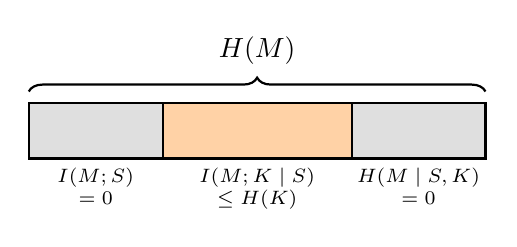
\begin{tikzpicture}
  \fill[gray!25] (0, 0) rectangle (1.7, 0.7);
  \fill[orange!35] (1.7, 0) rectangle (4.1, 0.7);
  \fill[gray!25] (4.1, 0) rectangle (5.8, 0.7);
  \draw[thick] (0, 0) rectangle (5.8, 0.7);
  \draw[thick] (1.7, 0) -- (1.7, 0.7);
  \draw[thick] (4.1, 0) -- (4.1, 0.7);
  \draw[decorate, decoration={brace, amplitude=5pt}, thick] (0, 0.85) -- (5.8, 0.85)
    node[midway, above=6pt] {$H(M)$};
  \node[below, font=\scriptsize, align=center] at (0.85, 0) {$I(M; S)$ \\ $= 0$};
  \node[below, font=\scriptsize, align=center] at (2.9, 0) {$I(M; K \mid S)$ \\ $\leq H(K)$};
  \node[below, font=\scriptsize, align=center] at (4.95, 0) {$H(M \mid S, K)$ \\ $= 0$};
\end{tikzpicture}
\end{center}
\vspace{1em}
\begin{center}
\fbox{$H(M) \leq H(K)$}
\end{center}
\end{column}
\end{columns}

\note{
\begin{itemize}
\item Perfect hiddenness: the observed stegotext reveals no information about the payload
\item This follows from perfect security: if $S = C$ for every payload, the stegotext does not depend on $M$
\item Perfect decoding: the receiver recovers $M$ exactly from the stegotext and the key
\item First line is the definition of mutual information, second line is the chain rule
\item Mutual information is bounded by entropy: $I(M; K \mid S) \leq H(K \mid S) \leq H(K)$
\item The picture: the entropy of the payload splits into three parts, two of them are forced to zero
\item Result: the shared secret must contain at least as much entropy as the payload
\end{itemize}
}
\end{frame}

\begin{frame}{Why This Is Impractical}
\begin{itemize}
\item The key has to grow linearly with the payload
\item Arbitrarily many payloads need an unbounded supply of shared randomness, or a way to refresh it
\item This is the one-time pad again: perfect secrecy consumes key material
\item Whoever can exchange that much secret randomness could often use that channel directly
\end{itemize}
\vspace{1em}
Steganography is still not useless: it hides the \textbf{existence} of communication, encryption only hides the \textbf{content}.

\vspace{1em}
Practical schemes use a short reusable key and settle for \textbf{computational security}.

\note{
\begin{itemize}
\item $H(M) \leq H(K)$ means the key length scales linearly with the payload length
\item A finite fixed key is not enough for arbitrarily many payloads
\item Analogous to the one-time pad
\item If sender and receiver already have a secret channel for large amounts of fresh randomness, they could often use it directly for communication or key refreshment
\item That does not make steganography useless, since it hides the existence of communication
\item But perfect information-theoretic steganography is usually expensive in secret randomness
\item So practical schemes use a short reusable key
\end{itemize}
}
\end{frame}

\begin{frame}{Computational Security}
Weaken the requirement:
\vspace{0.5em}
\begin{columns}[T]
\begin{column}{0.47\textwidth}
\textbf{Perfect}
\begin{itemize}
\item $S = C$
\item \emph{No one} can distinguish the two distributions
\end{itemize}
\end{column}
\begin{column}{0.47\textwidth}
\textbf{Computational}
\begin{itemize}
\item $S \approx C$ for efficient wardens
\item No \emph{polynomial-time} warden can distinguish them with non-negligible advantage
\end{itemize}
\end{column}
\end{columns}
\vspace{1.5em}
\begin{center}
An unbounded warden may still break the scheme.
\end{center}

\note{
\begin{itemize}
\item Instead of demanding $S = C$ against all wardens, we demand that no efficient warden can distinguish $S$ from $C$
\item The guarantee is not: no one can distinguish the two distributions
\item It is: no polynomial-time warden can distinguish them with non-negligible advantage
\item This is a reasonable assumption about real wardens
\item An unbounded warden may still break the scheme
\end{itemize}
}
\end{frame}

\begin{frame}{Pseudorandom Functions}
A \textbf{PRF} is a family of keyed functions
$$F_k : \{0,1\}^{\ell_1} \to \{0,1\}^{\ell_2}, \qquad \text{one for each key } k \in \{0,1\}^{\lambda}$$
\begin{enumerate}
\item $F_k$ is efficiently computable given $k$
\item For every polynomial-time distinguisher $D$ and a truly random function $f$:
$$\tfrac{1}{2} \Pr_{k \sim \mathrm{Unif}(\{0,1\}^\lambda)}\big[\, D^{F_k} = 0 \,\big] + \tfrac{1}{2} \Pr_{f}\big[\, D^{f} = 1 \,\big] \leq \tfrac{1}{2} + \mathrm{negl}(\lambda)$$
$$\text{where } \forall c > 0 \;\, \exists N \;\, \forall \lambda > N : \;\; \mathrm{negl}(\lambda) < \lambda^{-c}$$
\end{enumerate}
\vspace{0.5em}
A short key, but to efficient algorithms it looks like a truly random function.

\note{
\begin{itemize}
\item $\lambda$ is the key length, input and output lengths are polynomial in $\lambda$
\item The distinguisher gets oracle access: it can query the function but does not see the key
\item $f$ is a truly random function with the same domain and range
\item Intuition: a truly random function requires an enormous amount of randomness
\item A PRF uses only a short key
\item But to efficient algorithms it looks like a truly random function
\end{itemize}
}
\end{frame}

\begin{frame}{Assumptions and Attack Cost}
\begin{columns}[T]
\begin{column}{0.47\textwidth}
\textbf{Assumption}
\begin{itemize}
\item One-way functions exist
\item This implies that PRFs exist
\item $P \neq NP$ alone is too weak for modern cryptography
\end{itemize}
\vspace{0.5em}
\textbf{Security argument}
\begin{enumerate}
\item Assume secure PRFs exist
\item Replace true randomness by PRF output
\item Efficient wardens cannot tell the difference
\item So they cannot tell stegotext from covertext
\end{enumerate}
\end{column}
\begin{column}{0.47\textwidth}
\textbf{Attack cost}
\begin{itemize}
\item Generic attack: try all keys of length $\lambda$
$$O(2^\lambda)$$
\item For each key, check whether the text has the expected statistical structure
\item A weak PRF or a flawed construction allows faster attacks
\item A good scheme makes exhaustive search the best strategy
\end{itemize}
\end{column}
\end{columns}

\note{
\begin{itemize}
\item The relevant assumption is not simply $P \neq NP$, that is too weak for modern cryptography
\item The standard assumption is the existence of one-way functions, which implies the existence of PRFs
\item Go through the four steps of the security argument
\item Efficient wardens cannot distinguish stegotext from covertext, except with negligible advantage
\item Brute force: for each candidate key the warden checks whether the observed text has the statistical structure expected under that key
\item If the correct key is found, the warden can run the retrieval algorithm and decode the payload
\item The attack cost is at most $2^\lambda$ by exhaustive search
\item An unbounded warden can still brute-force the key
\end{itemize}
}
\end{frame}

\begin{frame}{Summary: The Trade-off}
\begin{center}
\renewcommand{\arraystretch}{1.4}
\begin{tabular}{lll}
\toprule
 & \textbf{Perfect} & \textbf{Computational} \\
\midrule
Guarantee & $S = C$ & no efficient distinguisher \\
Key & $H(K) \geq H(M)$, fresh & short, reusable \\
Assumption & none & secure PRFs exist \\
Unbounded warden & still secure & breaks it, cost up to $2^\lambda$ \\
\bottomrule
\end{tabular}
\end{center}

\note{
\begin{itemize}
\item Perfect information-theoretic steganography requires the stegotext distribution to equal the covertext distribution exactly
\item With perfect decoding it requires $H(K) \geq H(M)$
\item So unlimited perfect hidden communication requires an unlimited or refreshed secret resource
\item Computational steganography uses a short reusable key and a PRF
\item The output is computationally indistinguishable from covertext, assuming the PRF is secure
\item Practical, but only against efficient wardens
\end{itemize}
}
\end{frame}
